\chapter{La radioactivité}

\textit{La radioactivité est un phénomène naturel ou artificiel par lequel certains noyaux atomiques instables se transforment spontanément en d'autres noyaux, en émettant des particules et de l'énergie. Découverte à la fin du XIX\ieme{} siècle par Henri Becquerel, puis étudiée par Pierre et Marie Curie, elle est à la base de nombreuses applications en médecine (radiothérapie, imagerie), en datation (archéologie, géologie) et en production d'énergie (centrales nucléaires). Ce chapitre présente les lois fondamentales qui régissent la stabilité des noyaux, les différents types de radioactivité, la cinétique de la désintégration, ainsi que les réactions nucléaires provoquées.}

% ===================================================================
\section{Le noyau atomique et sa stabilité}

\subsection{Constituants du noyau}
Le noyau atomique est constitué de \textbf{nucléons} : les \textbf{protons} (charge $+e$) et les \textbf{neutrons} (charge nulle). Un noyau est représenté par $\ce{^{A}_{Z}X}$, où :
\begin{itemize}
    \item $Z$ : numéro atomique (nombre de protons) ;
    \item $A$ : nombre de masse (nombre de nucléons) ;
    \item $N = A - Z$ : nombre de neutrons.
\end{itemize}

\begin{definition}[Isotopes]
Des isotopes sont des noyaux ayant le même nombre de protons $Z$ mais des nombres de masse $A$ différents (donc des nombres de neutrons différents). Par exemple, le carbone possède trois isotopes naturels : $\ce{^{12}_{6}C}$, $\ce{^{13}_{6}C}$ et $\ce{^{14}_{6}C}$.
\end{definition}

\subsection{Stabilité nucléaire et diagramme $(N,Z)$}
La stabilité d'un noyau dépend de l'équilibre entre la répulsion électrostatique des protons et l'attraction nucléaire forte qui lie les nucléons. Les noyaux stables se situent dans une bande étroite appelée \textbf{valiée de stabilité} sur le diagramme $(N,Z)$.

\begin{illus}
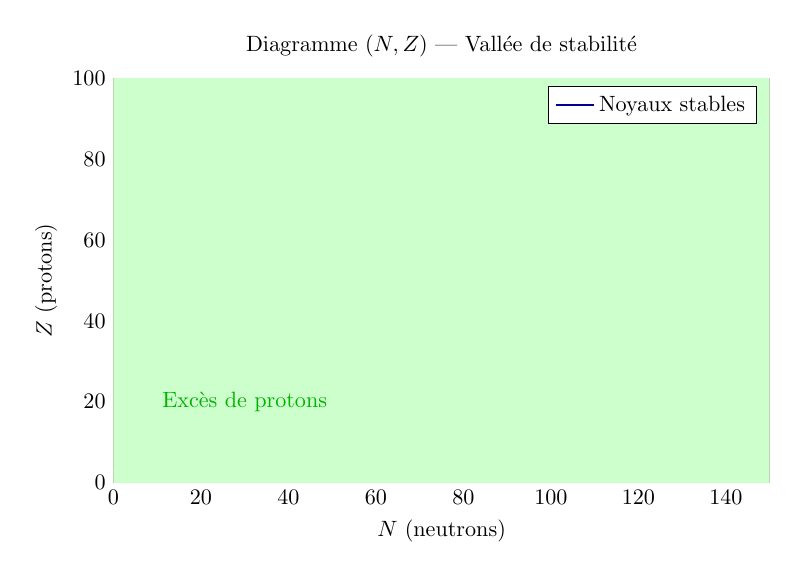
\begin{tikzpicture}[scale=0.8]
    \begin{axis}[
        xlabel={$N$ (neutrons)},
        ylabel={$Z$ (protons)},
        xmin=0, xmax=150,
        ymin=0, ymax=100,
        grid=both,
        width=12cm, height=8cm,
        title={Diagramme $(N,Z)$ — Vallée de stabilité}
    ]
        % Vallée de stabilité (bande)
        \addplot[domain=0:150, samples=200, thick, blue!60!black] {x/(1+0.007*x^(2/3))};
        \addplot[domain=0:150, samples=200, dashed, blue!40] {x/(1+0.007*x^(2/3))-3};
        \addplot[domain=0:150, samples=200, dashed, blue!40] {x/(1+0.007*x^(2/3))+3};
        \addlegendentry{Noyaux stables}
        % Zone excès de neutrons
        \fill[red!20] (0,0) -- (150,0) -- (150,100) -- (0,100) -- cycle;
        \node[red!70!black] at (120,80) {Excès de neutrons};
        % Zone excès de protons
        \fill[green!20] (0,0) -- (150,0) -- (150,100) -- (0,100) -- cycle;
        \node[green!70!black] at (30,20) {Excès de protons};
    \end{axis}
\end{tikzpicture}
\fig{Diagramme $(N,Z)$ montrant la vallée de stabilité (bande bleue). Les noyaux instables se désintègrent par radioactivité $\beta^-$ (excès de neutrons) ou $\beta^+$ (excès de protons).}
\end{illus}

\begin{propriete}[Stabilité]
Un noyau est d'autant plus stable que son énergie de liaison par nucléon est élevée. Les noyaux les plus stables se situent autour du fer ($\ce{^{56}_{26}Fe}$).
\end{propriete}

% ===================================================================
\section{Les différents types de radioactivité}

\subsection{Lois de conservation (Soddy)}
Lors d'une désintégration radioactive, deux grandeurs se conservent :
\begin{itemize}
    \item le nombre de masse $A$ ;
    \item la charge électrique $Z$.
\end{itemize}
Ces lois permettent d'écrire l'équation de la réaction nucléaire.

\subsection{Radioactivité $\alpha$}
\begin{definition}[Radioactivité alpha]
Un noyau instable émet une particule $\alpha$, qui est un noyau d'hélium $\ce{^{4}_{2}He}$. La réaction s'écrit :
\[\ce{^{A}_{Z}X -> ^{A-4}_{Z-2}Y + ^{4}_{2}He}\]
\end{definition}
\begin{exemple}
Le radium $\ce{^{226}_{88}Ra}$ se désintègre en radon $\ce{^{222}_{86}Rn}$ :
\[\ce{^{226}_{88}Ra -> ^{222}_{86}Rn + ^{4}_{2}He}\]
\end{exemple}

\subsection{Radioactivité $\beta^-$}
\begin{definition}[Radioactivité bêta moins]
Un neutron se transforme en proton avec émission d'un électron $\beta^-$ et d'un antineutrino $\bar{\nu}_e$ :
\[\ce{^{A}_{Z}X -> ^{A}_{Z+1}Y} + e^- + \bar{\nu}_e\]
\end{definition}

\subsection{Radioactivité $\beta^+$}
\begin{definition}[Radioactivité bêta plus]
Un proton se transforme en neutron avec émission d'un positon $\beta^+$ et d'un neutrino $\nu_e$ :
\[\ce{^{A}_{Z}X -> ^{A}_{Z-1}Y} + e^+ + \nu_e\]
\end{definition}

\subsection{Radioactivité $\gamma$}
\begin{definition}[Rayonnement gamma]
Un noyau excité (noté $\ce{^{A}_{Z}X^*}$) retourne à son état fondamental en émettant un photon $\gamma$ de haute énergie :
\[\ce{^{A}_{Z}X^* -> ^{A}_{Z}X} + \gamma\]
\end{definition}
\begin{remarque}
Le rayonnement $\gamma$ accompagne souvent les désintégrations $\alpha$ ou $\beta$ lorsque le noyau fils est formé dans un état excité.
\end{remarque}

% ===================================================================
\section{Familles radioactives}

Une famille radioactive est une séquence de noyaux instables qui se désintègrent successivement jusqu'à un noyau stable. On distingue quatre familles naturelles :
\begin{itemize}
    \item famille de l'uranium ($\ce{^{238}_{92}U}$) → plomb $\ce{^{206}_{82}Pb}$ ;
    \item famille du thorium ($\ce{^{232}_{90}Th}$) → plomb $\ce{^{208}_{82}Pb}$ ;
    \item famille de l'actinium ($\ce{^{235}_{92}U}$) → plomb $\ce{^{207}_{82}Pb}$ ;
    \item famille du neptunium ($\ce{^{237}_{93}Np}$) → bismuth $\ce{^{209}_{83}Bi}$ (artificielle).
\end{itemize}

\begin{illus}
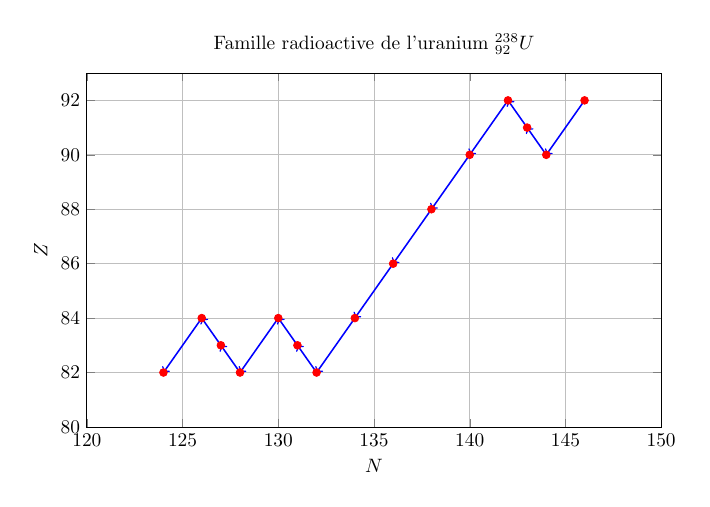
\begin{tikzpicture}[scale=0.7, transform shape]
    \begin{axis}[
        xlabel={$N$},
        ylabel={$Z$},
        xmin=120, xmax=150,
        ymin=80, ymax=93,
        grid=both,
        width=12cm, height=8cm,
        title={Famille radioactive de l'uranium $\ce{^{238}_{92}U}$}
    ]
        % Points de la famille (simplifiée)
        \addplot[only marks, mark=*, mark size=2pt, color=red] coordinates {
            (146,92)  % U-238
            (144,90)  % Th-234
            (143,91)  % Pa-234
            (142,92)  % U-234
            (140,90)  % Th-230
            (138,88)  % Ra-226
            (136,86)  % Rn-222
            (134,84)  % Po-218
            (132,82)  % Pb-214
            (131,83)  % Bi-214
            (130,84)  % Po-214
            (128,82)  % Pb-210
            (127,83)  % Bi-210
            (126,84)  % Po-210
            (124,82)  % Pb-206 (stable)
        };
        % Flèches (simulées par des segments)
        \addplot[->, thick, blue] coordinates {(146,92) (144,90)};
        \addplot[->, thick, blue] coordinates {(144,90) (143,91)};
        \addplot[->, thick, blue] coordinates {(143,91) (142,92)};
        \addplot[->, thick, blue] coordinates {(142,92) (140,90)};
        \addplot[->, thick, blue] coordinates {(140,90) (138,88)};
        \addplot[->, thick, blue] coordinates {(138,88) (136,86)};
        \addplot[->, thick, blue] coordinates {(136,86) (134,84)};
        \addplot[->, thick, blue] coordinates {(134,84) (132,82)};
        \addplot[->, thick, blue] coordinates {(132,82) (131,83)};
        \addplot[->, thick, blue] coordinates {(131,83) (130,84)};
        \addplot[->, thick, blue] coordinates {(130,84) (128,82)};
        \addplot[->, thick, blue] coordinates {(128,82) (127,83)};
        \addplot[->, thick, blue] coordinates {(127,83) (126,84)};
        \addplot[->, thick, blue] coordinates {(126,84) (124,82)};
    \end{axis}
\end{tikzpicture}
\fig{Famille radioactive de l'uranium $\ce{^{238}_{92}U}$ jusqu'au plomb $\ce{^{206}_{82}Pb}$. Chaque flèche représente une désintégration $\alpha$ ou $\beta$.}
\end{illus}

% ===================================================================
\section{Loi de décroissance radioactive}

\subsection{Loi statistique}
La désintégration d'un noyau est un phénomène aléatoire. Pour un échantillon contenant $N(t)$ noyaux radioactifs à l'instant $t$, le nombre de désintégrations par unité de temps est proportionnel au nombre de noyaux présents :
\[\dv{N}{t} = -\lambda N\]
où $\lambda$ est la \textbf{constante radioactive} (en $\si{\per\second}$).

\begin{loi}[Loi de décroissance exponentielle]
La solution de l'équation différentielle est :
\[N(t) = N_0 e^{-\lambda t}\]
où $N_0$ est le nombre de noyaux à $t=0$.
\end{loi}

\begin{illus}
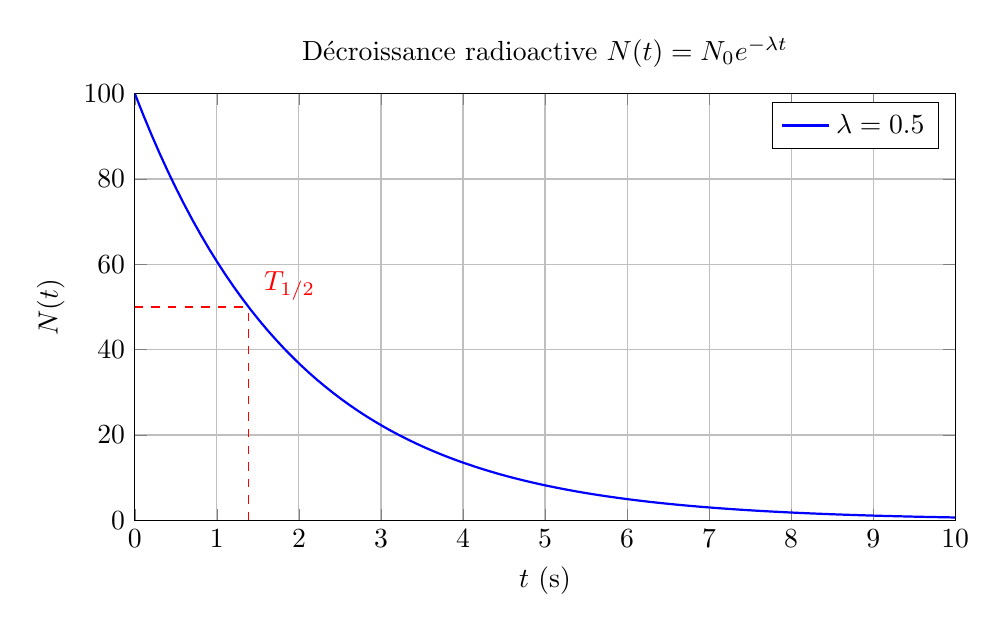
\begin{tikzpicture}
    \begin{axis}[
        xlabel={$t$ (s)},
        ylabel={$N(t)$},
        xmin=0, xmax=10,
        ymin=0, ymax=100,
        grid=both,
        width=12cm, height=7cm,
        title={Décroissance radioactive $N(t)=N_0 e^{-\lambda t}$}
    ]
        \addplot[domain=0:10, samples=100, thick, blue] {100*exp(-0.5*x)};
        \addlegendentry{$\lambda = \SI{0.5}{\per\second}$};
        % Demi-vie
        \draw[dashed, red] (axis cs:{ln(2)/0.5},0) -- (axis cs:{ln(2)/0.5},{50});
        \draw[dashed, red] (axis cs:0,50) -- (axis cs:{ln(2)/0.5},50);
        \node[red] at (axis cs:{ln(2)/0.5+0.5},55) {$T_{1/2}$};
    \end{axis}
\end{tikzpicture}
\fig{Courbe de décroissance exponentielle. La demi-vie $T_{1/2}$ est le temps au bout duquel la moitié des noyaux se sont désintégrés.}
\end{illus}

\subsection{Demi-vie}
\begin{definition}[Demi-vie]
La demi-vie $T_{1/2}$ (ou période radioactive) est le temps nécessaire pour que la moitié des noyaux initialement présents se désintègre. Elle est liée à $\lambda$ par :
\[T_{1/2} = \frac{\ln 2}{\lambda}\]
\end{definition}

\subsection{Activité}
\begin{definition}[Activité]
L'activité $A(t)$ d'un échantillon est le nombre de désintégrations par seconde :
\[A(t) = -\dv{N}{t} = \lambda N(t) = A_0 e^{-\lambda t}\]
L'unité est le \textbf{becquerel} (Bq) : $\SI{1}{\becquerel} = \SI{1}{\per\second}$.
\end{definition}

\subsection{Datation radioactive}
La datation par le carbone 14 repose sur la mesure de l'activité résiduelle d'un échantillon organique. En comparant l'activité actuelle $A$ à l'activité initiale $A_0$ (celle d'un organisme vivant), on détermine l'âge $t$ :
\[t = \frac{1}{\lambda} \ln\left(\frac{A_0}{A}\right) = \frac{T_{1/2}}{\ln 2} \ln\left(\frac{A_0}{A}\right)\]

\begin{exemple}
Un fragment de bois fossile a une activité de $\SI{0.23}{\becquerel}$ par gramme de carbone, alors qu'un arbre vivant a une activité de $\SI{0.23}{\becquerel}$ par gramme. Sachant que $T_{1/2}(\ce{^{14}C}) = \SI{5730}{ans}$, on trouve :
\[t = \frac{5730}{\ln 2} \ln\left(\frac{0.23}{0.23}\right) = 0\]
L'échantillon est donc contemporain (cas fictif où l'activité n'a pas diminué).
\end{exemple}

% ===================================================================
\section{Réactions nucléaires provoquées}

\subsection{Fission nucléaire}
\begin{definition}[Fission]
La fission est la rupture d'un noyau lourd (comme l'uranium $\ce{^{235}_{92}U}$) en deux noyaux plus légers, sous l'impact d'un neutron, avec libération d'énergie et de neutrons :
\[\ce{^{235}_{92}U + ^{1}_{0}n -> ^{141}_{56}Ba + ^{92}_{36}Kr + 3 ^{1}_{0}n + \text{énergie}}\]
\end{definition}

\subsection{Fusion nucléaire}
\begin{definition}[Fusion]
La fusion est l'union de deux noyaux légers pour former un noyau plus lourd, avec libération d'énergie. Par exemple, la fusion du deutérium et du tritium :
\[\ce{^{2}_{1}H + ^{3}_{1}H -> ^{4}_{2}He + ^{1}_{0}n + \text{énergie}}\]
\end{definition}

\subsection{Énergie de liaison et défaut de masse}
\begin{definition}[Défaut de masse]
La masse d'un noyau $\ce{^{A}_{Z}X}$ est inférieure à la somme des masses de ses nucléons isolés. Le défaut de masse $\Delta m$ est :
\[\Delta m = Z m_p + (A-Z) m_n - m_{\text{noyau}}\]
où $m_p$ et $m_n$ sont les masses du proton et du neutron.
\end{definition}

\begin{loi}[Énergie de liaison]
L'énergie de liaison $E_l$ est l'énergie qu'il faut fournir pour dissocier le noyau en ses nucléons. Elle est donnée par la relation d'Einstein :
\[E_l = \Delta m \cdot c^2\]
où $c = \SI{3.00e8}{\metre\per\second}$.
\end{loi}

\begin{illus}
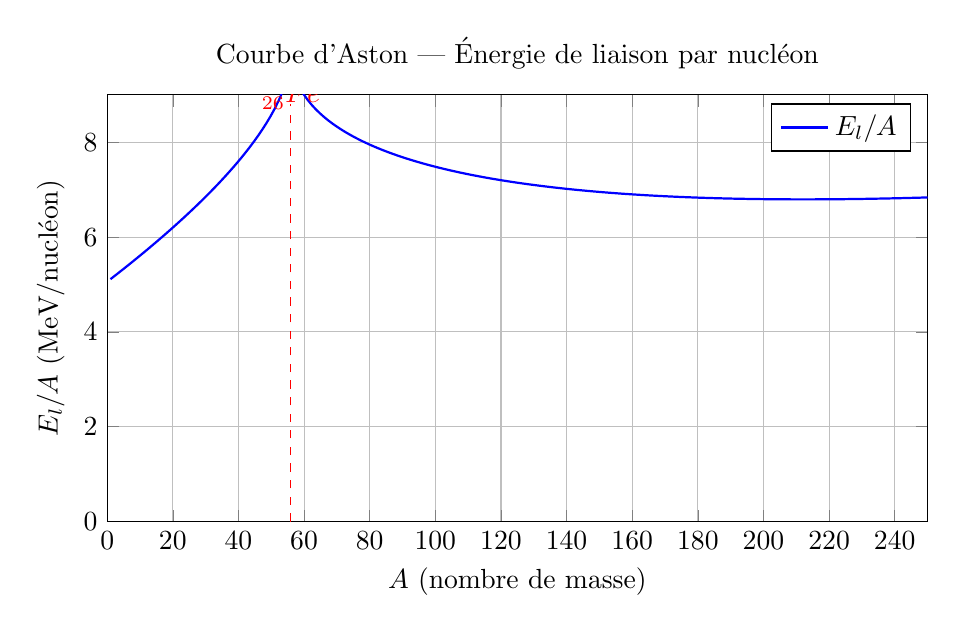
\begin{tikzpicture}
    \begin{axis}[
        xlabel={$A$ (nombre de masse)},
        ylabel={$E_l/A$ (MeV/nucléon)},
        xmin=0, xmax=250,
        ymin=0, ymax=9,
        grid=both,
        width=12cm, height=7cm,
        title={Courbe d'Aston — Énergie de liaison par nucléon}
    ]
        \addplot[domain=1:250, samples=200, thick, blue] {8.8 - 0.5*abs(x-56)^0.5 + 0.02*x};
        \addlegendentry{$E_l/A$}
        \draw[dashed, red] (axis cs:56,0) -- (axis cs:56,8.8);
        \node[red] at (axis cs:56,9) {$\ce{^{56}_{26}Fe}$};
    \end{axis}
\end{tikzpicture}
\fig{Courbe d'Aston : l'énergie de liaison par nucléon est maximale pour le fer $\ce{^{56}_{26}Fe}$. Les noyaux légers (fusion) et lourds (fission) peuvent libérer de l'énergie en se rapprochant du maximum.}
\end{illus}

\begin{aretenir}
La fission et la fusion libèrent de l'énergie car les noyaux produits ont une énergie de liaison par nucléon plus élevée que les noyaux de départ. La fusion libère davantage d'énergie par unité de masse que la fission.
\end{aretenir}

% ===================================================================
\section{L'essentiel à retenir}

\begin{synthese}
\paragraph{Lois de conservation (Soddy)} : $A$ et $Z$ se conservent dans toute réaction nucléaire.

\paragraph{Types de radioactivité}
\begin{itemize}
    \item $\alpha$ : $\ce{^{A}_{Z}X -> ^{A-4}_{Z-2}Y + ^{4}_{2}He}$
    \item $\beta^-$ : $\ce{^{A}_{Z}X -> ^{A}_{Z+1}Y} + e^- + \bar{\nu}_e$
    \item $\beta^+$ : $\ce{^{A}_{Z}X -> ^{A}_{Z-1}Y} + e^+ + \nu_e$
    \item $\gamma$ : $\ce{^{A}_{Z}X^* -> ^{A}_{Z}X} + \gamma$
\end{itemize}

\paragraph{Loi de décroissance} : $N(t) = N_0 e^{-\lambda t}$, $T_{1/2} = \frac{\ln 2}{\lambda}$, $A(t) = \lambda N(t)$.

\paragraph{Énergie nucléaire} : $E_l = \Delta m \cdot c^2$, avec $\Delta m = Z m_p + (A-Z) m_n - m_{\text{noyau}}$.

\paragraph{Applications} : datation ($\ce{^{14}C}$), fission (centrales), fusion (étoiles).

\paragraph{Unités} : $\lambda$ en $\si{\per\second}$, $T_{1/2}$ en secondes (ou années), $A$ en becquerels ($\si{\becquerel}$), $E_l$ en joules ou MeV ($\SI{1}{\MeV} = \SI{1.60e-13}{\joule}$).
\end{synthese}

% ===================================================================
\section{Méthodes \& savoir-faire}

\methode{Écrire une équation de désintégration}
Utiliser les lois de conservation de $A$ et $Z$. Identifier le type de radioactivité d'après la particule émise ($\alpha$, $\beta^-$, $\beta^+$, $\gamma$).

\begin{exemple}
Le polonium $\ce{^{210}_{84}Po}$ se désintègre en émettant une particule $\alpha$. Écrire l'équation.
\corrige{de la méthode}
$\ce{^{210}_{84}Po -> ^{206}_{82}Pb + ^{4}_{2}He}$ (vérification : $210 = 206+4$, $84 = 82+2$).
\end{exemple}

\methode{Calculer la constante radioactive et la demi-vie}
Utiliser $T_{1/2} = \frac{\ln 2}{\lambda}$ ou $\lambda = \frac{\ln 2}{T_{1/2}}$.

\begin{exemple}
Le césium $\ce{^{137}_{55}Cs}$ a une demi-vie de $\SI{30}{ans}$. Calculer $\lambda$ en $\si{\per\second}$.
\corrige{de la méthode}
$\lambda = \frac{\ln 2}{30 \times 365 \times 24 \times 3600} \approx \SI{7.33e-10}{\per\second}$.
\end{exemple}

\methode{Utiliser la loi de décroissance}
Pour trouver $N(t)$ ou $t$, appliquer $N(t) = N_0 e^{-\lambda t}$.

\begin{exemple}
Un échantillon contient initialement $N_0 = \num{1.0e20}$ noyaux de $\ce{^{60}_{27}Co}$ ($T_{1/2} = \SI{5.27}{ans}$). Combien reste-t-il après $\SI{10}{ans}$ ?
\corrige{de la méthode}
$\lambda = \frac{\ln 2}{5.27} \approx \num{0.1316}~\mathrm{an}^{-1}$, $N(10) = \num{1.0e20} \times e^{-0.1316 \times 10} \approx \num{2.68e19}$ noyaux.
\end{exemple}

\methode{Calculer l'activité}
$A(t) = \lambda N(t)$. Attention aux unités : $\lambda$ en $\si{\per\second}$ donne $A$ en $\si{\becquerel}$.

\begin{exemple}
Pour l'échantillon précédent, calculer l'activité initiale.
\corrige{de la méthode}
$\lambda = \frac{\ln 2}{5.27 \times 365 \times 24 \times 3600} \approx \SI{4.17e-9}{\per\second}$, $A_0 = \lambda N_0 = \SI{4.17e-9}{\per\second} \times \num{1.0e20} = \SI{4.17e11}{\becquerel}$.
\end{exemple}

\methode{Dater un échantillon}
Utiliser $t = \frac{T_{1/2}}{\ln 2} \ln\left(\frac{A_0}{A}\right)$.

\begin{exemple}
Un échantillon de bois ancien a une activité de $\SI{0.115}{\becquerel}$ par gramme de carbone, alors qu'un arbre vivant a $\SI{0.230}{\becquerel}$ par gramme. $T_{1/2}(\ce{^{14}C}) = \SI{5730}{ans}$. Quel est l'âge ?
\corrige{de la méthode}
$t = \frac{5730}{\ln 2} \ln\left(\frac{0.230}{0.115}\right) = \frac{5730}{0.693} \times \ln 2 = \SI{5730}{ans}$.
\end{exemple}

\methode{Calculer l'énergie de liaison}
$\Delta m = Z m_p + (A-Z) m_n - m_{\text{noyau}}$, puis $E_l = \Delta m \cdot c^2$.

\begin{exemple}
Pour $\ce{^{4}_{2}He}$, $m_{\text{noyau}} = \SI{4.0015}{u}$, $m_p = \SI{1.0073}{u}$, $m_n = \SI{1.0087}{u}$. Calculer $E_l$ en MeV.
\corrige{de la méthode}
$\Delta m = 2 \times 1.0073 + 2 \times 1.0087 - 4.0015 = \SI{0.0305}{u}$. $1 u = \SI{931.5}{\MeV\per\clight\squared}$, donc $E_l = 0.0305 \times 931.5 \approx \SI{28.4}{\MeV}$.
\end{exemple}

\methode{Distinguer fission et fusion}
La fission concerne les noyaux lourds ($A > 200$), la fusion les noyaux légers ($A < 20$). Les deux libèrent de l'énergie.

\begin{exemple}
Identifier : $\ce{^{235}_{92}U + ^{1}_{0}n -> ^{141}_{56}Ba + ^{92}_{36}Kr + 3 ^{1}_{0}n}$.
\corrige{de la méthode}
C'est une fission car un noyau lourd se scinde en deux noyaux moyens.
\end{exemple}

% ===================================================================
\section{Exercices d'application}

\rubrique{Équations de désintégration}

\exo{}\diff{1} Écrire l'équation de désintégration $\alpha$ du radium $\ce{^{226}_{88}Ra}$.

\exo{}\diff{1} Le thorium $\ce{^{234}_{90}Th}$ se désintègre par émission $\beta^-$. Écrire l'équation.

\exo{}\diff{2} Le sodium $\ce{^{22}_{11}Na}$ se désintègre par $\beta^+$. Écrire l'équation et identifier le noyau fils.

\rubrique{Loi de décroissance}

\exo{}\diff{1} Un échantillon contient $N_0 = \num{5.0e18}$ noyaux de $\ce{^{131}_{53}I}$ ($T_{1/2} = \SI{8.02}{jours}$). Calculer $\lambda$ en $\si{\per\second}$.

\exo{}\diff{2} Pour l'échantillon précédent, calculer $N(t)$ après $\SI{24}{jours}$.

\exo{}\diff{2} L'activité initiale d'un échantillon de $\ce{^{60}_{27}Co}$ est $A_0 = \SI{1.0e9}{\becquerel}$. $T_{1/2} = \SI{5.27}{ans}$. Calculer l'activité après $\SI{10}{ans}$.

\rubrique{Datation}

\exo{}\diff{2} Un fossile a une activité $\ce{^{14}C}$ de $\SI{0.0575}{\becquerel}$ par gramme de carbone. $T_{1/2} = \SI{5730}{ans}$, $A_0 = \SI{0.230}{\becquerel}$. Quel est son âge ?

\exo{}\diff{3} Un échantillon de bois ancien a une activité de $\SI{0.02875}{\becquerel}$ par gramme. Déterminer son âge.

\rubrique{Énergie de liaison}

\exo{}\diff{2} Calculer le défaut de masse et l'énergie de liaison de $\ce{^{12}_{6}C}$. Données : $m_{\ce{^{12}C}} = \SI{12.0000}{u}$, $m_p = \SI{1.0073}{u}$, $m_n = \SI{1.0087}{u}$, $1 u = \SI{931.5}{\MeV\per\clight\squared}$.

\exo{}\diff{3} Pour $\ce{^{235}_{92}U}$, $m = \SI{235.0439}{u}$. Calculer $E_l$ par nucléon.

\rubrique{Fission et fusion}

\exo{}\diff{2} Écrire l'équation de fission de $\ce{^{235}_{92}U}$ avec un neutron donnant $\ce{^{141}_{56}Ba}$ et $\ce{^{92}_{36}Kr}$. Combien de neutrons sont émis ?

\exo{}\diff{3} La fusion $\ce{^{2}_{1}H + ^{3}_{1}H -> ^{4}_{2}He + ^{1}_{0}n}$ libère $\SI{17.6}{\MeV}$. Calculer l'énergie libérée par nucléon de deutérium.

% ===================================================================
\section{Exercices d'entraînement}

\rubrique{Équations de désintégration}

\exo{}\diff{1} Compléter : $\ce{^{238}_{92}U -> ^{234}_{90}Th} + ?$.

\exo{}\diff{2} Le bismuth $\ce{^{210}_{83}Bi}$ se désintègre par $\beta^-$. Écrire l'équation.

\exo{}\diff{2} Le carbone $\ce{^{11}_{6}C}$ se désintègre par $\beta^+$. Écrire l'équation.

\exo{}\diff{1} Identifier le type de radioactivité : $\ce{^{60}_{27}Co -> ^{60}_{28}Ni} + e^- + \bar{\nu}_e$.

\exo{}\diff{2} Le polonium $\ce{^{210}_{84}Po}$ émet une particule $\alpha$. Quel est le noyau fils ?

\rubrique{Loi de décroissance}

\exo{}\diff{2} Un échantillon de $\ce{^{99}_{43}Tc}$ ($T_{1/2} = \SI{6.01}{h}$) contient $N_0 = \num{2.0e15}$ noyaux. Calculer $N$ après $\SI{12}{h}$.

\exo{}\diff{2} L'activité d'un échantillon de $\ce{^{131}_{53}I}$ est $A = \SI{3.0e6}{\becquerel}$ après $\SI{16}{jours}$. $T_{1/2} = \SI{8.02}{jours}$. Calculer $A_0$.

\exo{}\diff{3} Un échantillon radioactif a une activité de $\SI{500}{\becquerel}$ à $t=0$ et de $\SI{125}{\becquerel}$ après $\SI{12}{h}$. Calculer $T_{1/2}$.

\exo{}\diff{2} Le radon $\ce{^{222}_{86}Rn}$ a $T_{1/2} = \SI{3.82}{jours}$. Quelle fraction reste après $\SI{10}{jours}$ ?

\rubrique{Datation}

\exo{}\diff{2} Un os fossile a une activité $\ce{^{14}C}$ de $\SI{0.0115}{\becquerel}$ par gramme. $A_0 = \SI{0.230}{\becquerel}$. Quel est son âge ?

\exo{}\diff{3} Un échantillon de charbon de bois a une activité de $\SI{0.046}{\becquerel}$ par gramme. Déterminer l'âge.

\rubrique{Énergie de liaison}

\exo{}\diff{2} Calculer $E_l$ pour $\ce{^{56}_{26}Fe}$ ($m = \SI{55.9349}{u}$).

\exo{}\diff{3} Comparer $E_l/A$ pour $\ce{^{4}_{2}He}$ et $\ce{^{235}_{92}U}$.

\rubrique{Fission et fusion}

\exo{}\diff{2} Écrire l'équation de fission de $\ce{^{235}_{92}U}$ avec un neutron donnant $\ce{^{94}_{38}Sr}$ et $\ce{^{139}_{54}Xe}$.

\exo{}\diff{3} La fusion de $\ce{^{2}_{1}H}$ et $\ce{^{3}_{1}H}$ libère $\SI{17.6}{\MeV}$. Combien de fusions sont nécessaires pour produire $\SI{1}{\kilo\watt\hour}$ ?

\exo{}\diff{2} Expliquer pourquoi la fusion est plus difficile à réaliser que la fission sur Terre.

% ===================================================================
\section{Sujets type Baccalauréat}

\sujetbac[Datation au carbone 14]
Un fragment de bois fossile est découvert lors de fouilles archéologiques à Yaoundé. On mesure son activité $\ce{^{14}C}$ : $A = \SI{0.0575}{\becquerel}$ par gramme de carbone. L'activité d'un organisme vivant est $A_0 = \SI{0.230}{\becquerel}$ par gramme. La demi-vie du $\ce{^{14}C}$ est $T_{1/2} = \SI{5730}{ans}$.

\begin{enumerate}[label=\arabic*)]
    \item Définir la demi-vie.
    \item Calculer la constante radioactive $\lambda$ du $\ce{^{14}C}$ en $\mathrm{an}^{-1}$.
    \item Déterminer l'âge du fossile.
    \item Si l'incertitude sur la mesure de $A$ est de $\pm \SI{5}{\percent}$, donner un encadrement de l'âge.
\end{enumerate}

\sujetbac[Énergie de fission]
Dans une centrale nucléaire, la fission de l'uranium $\ce{^{235}_{92}U}$ est utilisée. Une réaction possible est :
\[\ce{^{235}_{92}U + ^{1}_{0}n -> ^{94}_{38}Sr + ^{139}_{54}Xe + 3 ^{1}_{0}n}\]
Données : $m(\ce{^{235}_{92}U}) = \SI{235.0439}{u}$, $m(\ce{^{94}_{38}Sr}) = \SI{93.9154}{u}$, $m(\ce{^{139}_{54}Xe}) = \SI{138.9188}{u}$, $m_n = \SI{1.0087}{u}$, $1 u = \SI{931.5}{\MeV\per\clight\squared}$.

\begin{enumerate}[label=\arabic*)]
    \item Vérifier la conservation du nombre de masse et de la charge.
    \item Calculer le défaut de masse $\Delta m$ de la réaction en unité de masse atomique.
    \item En déduire l'énergie libérée par une fission en MeV, puis en joules.
    \item Une centrale fournit une puissance électrique de $\SI{900}{\mega\watt}$ avec un rendement de $\SI{33}{\percent}$. Calculer la masse d'uranium consommée par jour.
\end{enumerate}

\sujetbac[Famille radioactive]
On considère la famille radioactive du thorium $\ce{^{232}_{90}Th}$. Le thorium se désintègre par $\alpha$ en radium $\ce{^{228}_{88}Ra}$, qui lui-même se désintègre par $\beta^-$ en actinium $\ce{^{228}_{89}Ac}$.

\begin{enumerate}[label=\arabic*)]
    \item Écrire les équations de ces deux désintégrations.
    \item L'actinium se désintègre à son tour par $\beta^-$. Écrire l'équation et identifier le noyau fils.
    \item Le noyau fils précédent se désintègre par $\alpha$. Écrire l'équation.
    \item Montrer que le thorium $\ce{^{232}_{90}Th}$ et le plomb $\ce{^{208}_{82}Pb}$ sont reliés par une série de désintégrations. Combien de désintégrations $\alpha$ et $\beta$ sont nécessaires ?
\end{enumerate}

% ===================================================================
\section{Corrigés}

\corrige{de l'exercice 1}
$\ce{^{226}_{88}Ra -> ^{222}_{86}Rn + ^{4}_{2}He}$

\corrige{de l'exercice 2}
$\ce{^{234}_{90}Th -> ^{234}_{91}Pa} + e^- + \bar{\nu}_e$

\corrige{de l'exercice 3}
$\ce{^{22}_{11}Na -> ^{22}_{10}Ne} + e^+ + \nu_e$

\corrige{de l'exercice 4}
$\lambda = \frac{\ln 2}{8.02 \times 24 \times 3600} \approx \SI{1.00e-6}{\per\second}$

\corrige{de l'exercice 5}
$\lambda = \frac{\ln 2}{8.02} \approx \SI{0.0864}{\per\day}$, $N(24) = \num{5.0e18} \times e^{-0.0864 \times 24} \approx \num{6.25e17}$

\corrige{de l'exercice 6}
$\lambda = \frac{\ln 2}{5.27} \approx \num{0.1316}~\mathrm{an}^{-1}$, $A(10) = \SI{1.0e9}{\becquerel} \times e^{-0.1316 \times 10} \approx \SI{2.68e8}{\becquerel}$

\corrige{de l'exercice 7}
$t = \frac{5730}{\ln 2} \ln\left(\frac{0.230}{0.0575}\right) = \frac{5730}{0.693} \times \ln 4 \approx \SI{11460}{ans}$

\corrige{de l'exercice 8}
$t = \frac{5730}{\ln 2} \ln\left(\frac{0.230}{0.02875}\right) = \frac{5730}{0.693} \times \ln 8 \approx \SI{17190}{ans}$

\corrige{de l'exercice 9}
$\Delta m = 6 \times 1.0073 + 6 \times 1.0087 - 12.0000 = \SI{0.0960}{u}$, $E_l = 0.0960 \times 931.5 \approx \SI{89.4}{\MeV}$

\corrige{de l'exercice 10}
$\Delta m = 92 \times 1.0073 + 143 \times 1.0087 - 235.0439 = \SI{1.9150}{u}$, $E_l = 1.9150 \times 931.5 \approx \SI{1784}{\MeV}$, $E_l/A \approx \SI{7.59}{\MeV\per\nucleon}$

\corrige{de l'exercice 11}
$\ce{^{235}_{92}U + ^{1}_{0}n -> ^{141}_{56}Ba + ^{92}_{36}Kr + 3 ^{1}_{0}n}$ (3 neutrons émis)

\corrige{de l'exercice 12}
Énergie par nucléon de deutérium : $\frac{17.6}{2} = \SI{8.8}{\MeV\per\nucleon}$

\corrige{du sujet 1}
1. La demi-vie est le temps au bout duquel la moitié des noyaux initialement présents se sont désintégrés.
2. $\lambda = \frac{\ln 2}{5730} \approx \num{1.21e-4}~\mathrm{an}^{-1}$
3. $t = \frac{5730}{\ln 2} \ln\left(\frac{0.230}{0.0575}\right) = \SI{11460}{ans}$
4. $A_{\min} = 0.0575 \times 0.95 = \SI{0.0546}{\becquerel}$, $A_{\max} = 0.0575 \times 1.05 = \SI{0.0604}{\becquerel}$ ; $t_{\min} = \frac{5730}{\ln 2} \ln\left(\frac{0.230}{0.0604}\right) \approx \SI{10900}{ans}$, $t_{\max} = \frac{5730}{\ln 2} \ln\left(\frac{0.230}{0.0546}\right) \approx \SI{12000}{ans}$.

\corrige{du sujet 2}
1. $A$ : $235+1 = 94+139+3 = 236$ ; $Z$ : $92+0 = 38+54+0 = 92$.
2. $\Delta m = (235.0439 + 1.0087) - (93.9154 + 138.9188 + 3 \times 1.0087) = \SI{0.1866}{u}$
3. $E = 0.1866 \times 931.5 \approx \SI{173.8}{\MeV} = 173.8 \times 1.60e-13 \approx \SI{2.78e-11}{\joule}$
4. Puissance thermique : $P_{\text{th}} = \frac{900}{0.33} \approx \SI{2727}{\mega\watt}$ ; énergie par jour : $E_{\text{jour}} = 2727 \times 10^6 \times 24 \times 3600 \approx \SI{2.36e14}{\joule}$ ; nombre de fissions : $N = \frac{2.36e14}{2.78e-11} \approx \num{8.49e24}$ ; masse : $m = \frac{8.49e24 \times 235.0439 \times 1.66e-27}{1000} \approx \SI{3.31}{\kilogram}$.

\corrige{du sujet 3}
1. $\ce{^{232}_{90}Th -> ^{228}_{88}Ra + ^{4}_{2}He}$ ; $\ce{^{228}_{88}Ra -> ^{228}_{89}Ac} + e^- + \bar{\nu}_e$
2. $\ce{^{228}_{89}Ac -> ^{228}_{90}Th} + e^- + \bar{\nu}_e$
3. $\ce{^{228}_{90}Th -> ^{224}_{88}Ra + ^{4}_{2}He}$
4. Pour passer de $\ce{^{232}_{90}Th}$ à $\ce{^{208}_{82}Pb}$, il faut perdre $24$ nucléons et $8$ protons. Chaque $\alpha$ perd $4$ nucléons et $2$ protons, chaque $\beta$ ne change pas $A$ mais augmente $Z$ de $1$. Soit $x$ désintégrations $\alpha$ et $y$ $\beta$ : $4x = 24 \Rightarrow x = 6$ ; $2x - y = 8 \Rightarrow y = 4$. Il faut $6$ $\alpha$ et $4$ $\beta$.